\documentclass{article}

% packages
\usepackage{amsmath, amsthm, thmtools, amsfonts, amssymb, luacode, catchfile, tikzducks, hyperref, ifthen}
\ifcsname c@kobocompile\endcsname
	\usepackage[a5paper, total={1072pt, 1448pt}, margin=10pt, includeheadfoot]{geometry} % set page margins
\else
	\usepackage[a4paper, margin=50pt, includeheadfoot]{geometry}
\fi
\usepackage[shortlabels]{enumitem}
\usepackage[skip=3pt, indent=0pt]{parskip}

% language
\usepackage[bidi=basic, layout=tabular, provide=*]{babel}
\ifcsname c@english\endcsname
	\babelprovide[main, import]{english}
\else
	\babelprovide[main, import]{hebrew}
	\babelprovide{rl}
\fi
%\babelfont{rm}{Libertinus Serif}
\babelfont{rm}[Renderer=Harfbuzz]{Libertinus Serif}
\babelfont{sf}{Libertinus Sans}
\babelfont{tt}{Libertinus Mono}

% style
\AddToHook{cmd/section/before}{\clearpage}	% Add line break before section
\linespread{1.3}
\setcounter{secnumdepth}{0}		% Remove default number tags from sections, this won't do well with theorems
\AtBeginDocument{\setlength{\belowdisplayskip}{3pt}}
\AtBeginDocument{\setlength{\abovedisplayskip}{3pt}}
\graphicspath{ {../images/} }

% operators
\DeclareMathOperator\cis{cis}
\DeclareMathOperator\Sp{Sp}
\DeclareMathOperator\tr{tr}
\DeclareMathOperator\im{Im}
\DeclareMathOperator\re{Re}
\DeclareMathOperator\diag{diag}
\DeclareMathOperator*\lowlim{\underline{lim}}
\DeclareMathOperator*\uplim{\overline{lim}}
\DeclareMathOperator\rng{rng}
\DeclareMathOperator\Sym{Sym}
\DeclareMathOperator\Arg{Arg}
\DeclareMathOperator\Log{Log}
\DeclareMathOperator\dom{dom}
\DeclareMathOperator\supp{Supp}
\DeclareMathOperator\var{Var}
\DeclareMathOperator\cov{Cov}

% commands
%\renewcommand\qedsymbol{\textbf{מש''ל}}
%\renewcommand\qedsymbol{\fbox{\emoji{lizard}}}
\newcommand{\Aa}[0]{\mathcal{A}}
\newcommand{\Bb}[0]{\mathcal{B}}
\newcommand{\CC}[0]{\mathbb{C}}
\newcommand{\Cc}[0]{\mathcal{C}}
\newcommand{\EE}[0]{\mathbb{E}}
\newcommand{\FF}[0]{\mathbb{F}}
\newcommand{\Ff}[0]{\mathcal{F}}
\newcommand{\Ii}[0]{\mathcal{I}}
\newcommand{\Gg}[0]{\mathcal{G}}
\newcommand{\Ll}[0]{\mathcal{L}}
\newcommand{\Mm}[0]{\mathcal{M}}
\newcommand{\NN}[0]{\mathbb{N}}
\newcommand{\Nn}[0]{\mathcal{N}}
\newcommand{\PP}[0]{\mathbb{P}}
\newcommand{\Pp}[0]{\mathcal{P}}
\newcommand{\QQ}[0]{\mathbb{Q}}
\newcommand{\RR}[0]{\mathbb{R}}
\newcommand{\Rr}[0]{\mathcal{R}}
\newcommand{\Ss}[0]{\mathcal{S}}
\newcommand{\TT}[0]{\mathbb{T}}
\newcommand{\Uu}[0]{\mathcal{U}}
\newcommand{\Vv}[0]{\mathcal{V}}
\newcommand{\Ww}[0]{\mathcal{W}}
\newcommand{\ZZ}[0]{\mathbb{Z}}
\newcommand{\acts}[0]{\circlearrowright}
\newcommand{\explain}[2] {
	\begin{flalign*}
		 && \text{#2} && \text{#1}
	\end{flalign*}
}
\newcommand{\maketitleprint}[0]{ \begin{center}
	%\begin{tikzpicture}[scale=3]
	%	\duck[graduate=gray!20!black, tassel=red!70!black]
	%\end{tikzpicture}	
	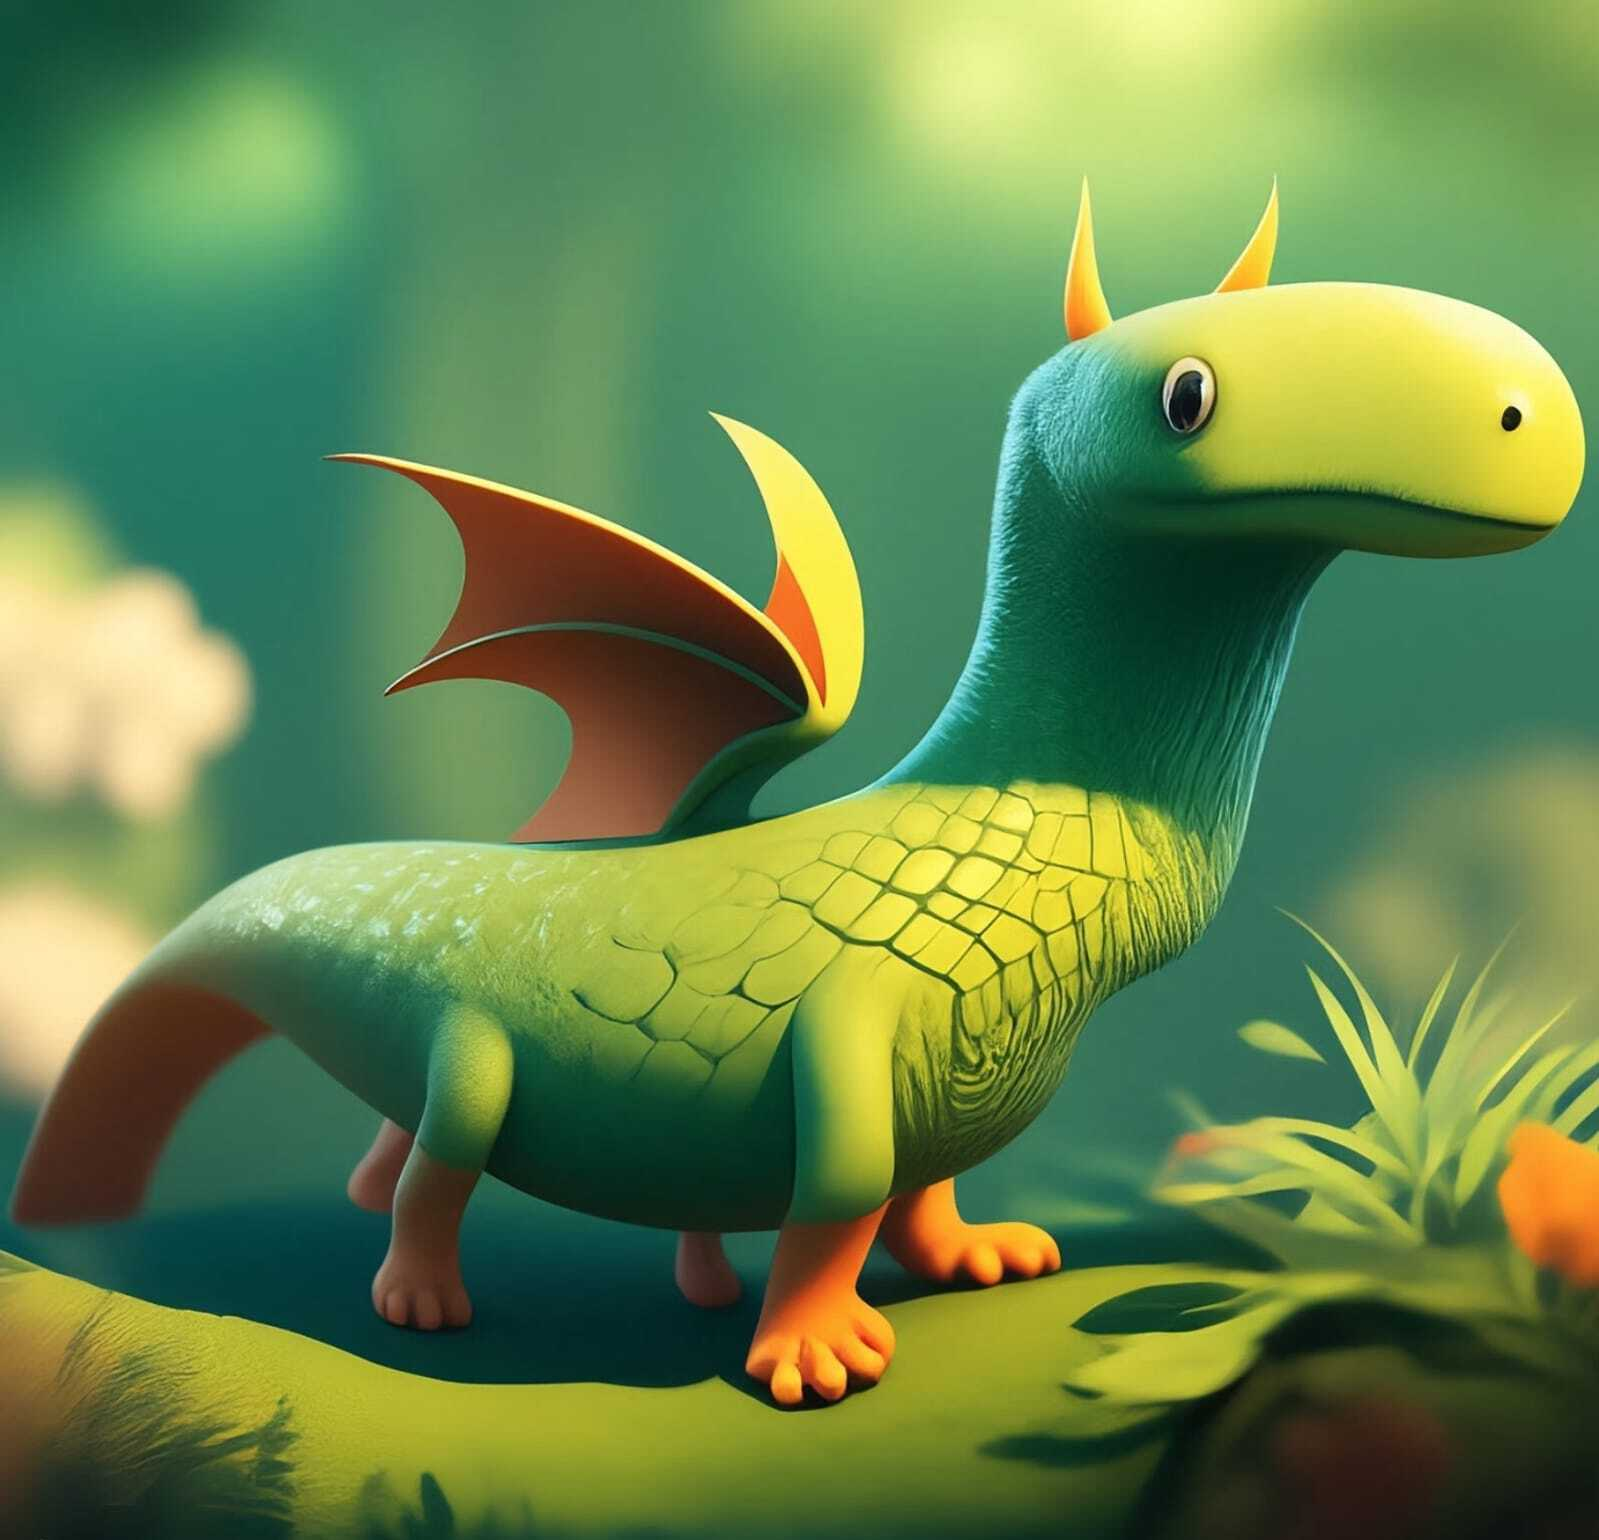
\includegraphics[width=6cm]{cover}
\end{center}
}

% theorem commands
\newtheoremstyle{c_remark}
	{}	% Space above
	{}	% Space below
	{}% Body font
	{}	% Indent amount
	{\bfseries}	% Theorem head font
	{}	% Punctuation after theorem head
	{.5em}	% Space after theorem head
	{\thmname{#1}\thmnumber{ #2}\thmnote{ \normalfont{\text{(#3)}}}}	% head content
\newtheoremstyle{c_definition}
	{3pt}	% Space above
	{3pt}	% Space below
	{}% Body font
	{}	% Indent amount
	{\bfseries}	% Theorem head font
	{}	% Punctuation after theorem head
	{.5em}	% Space after theorem head
	{\thmname{#1}\thmnumber{ #2}\thmnote{ \normalfont{\text{(#3)}}}}	% head content
\newtheoremstyle{c_plain}
	{3pt}	% Space above
	{3pt}	% Space below
	{\itshape}% Body font
	{}	% Indent amount
	{\bfseries}	% Theorem head font
	{}	% Punctuation after theorem head
	{.5em}	% Space after theorem head
	{\thmname{#1}\thmnumber{ #2}\thmnote{ \text{(#3)}}}	% head content

\ifcsname c@english\endcsname
	\theoremstyle{plain}
	\newtheorem{theorem}{Theorem}[section]
	\newtheorem{lemma}[theorem]{Lemma}
	\newtheorem{proposition}[theorem]{Proposition}
	\newtheorem*{proposition*}{Proposition}
	%\newtheorem{corollary}[theorem]{אין חלופה עברית}

	\theoremstyle{definition}
	\newtheorem{definition}[theorem]{Definition}
	\newtheorem*{definition*}{Definition}
	\newtheorem{example}{Example}[section]
	\newtheorem{exercise}{Exercise}[section]

	\theoremstyle{remark}
	\newtheorem*{remark}{Remark}
	\newtheorem*{solution}{Solution}
	\newtheorem{conclusion}[theorem]{Conclusion}
	\newtheorem{notation}[theorem]{Notation}
\else
	\theoremstyle{c_plain}
	\newtheorem{theorem}{משפט}[section]
	\newtheorem{lemma}[theorem]{למה}
	\newtheorem{proposition}[theorem]{טענה}
	\newtheorem*{proposition*}{טענה}
	%\newtheorem{corollary}[theorem]{אין חלופה עברית}

	\theoremstyle{c_definition}
	\newtheorem{definition}[theorem]{הגדרה}
	\newtheorem*{definition*}{הגדרה}
	\newtheorem{example}{דוגמה}[section]
	\newtheorem{exercise}{תרגיל}[section]

	\theoremstyle{c_remark}
	\newtheorem*{remark}{הערה}
	\newtheorem*{solution}{פתרון}
	\newtheorem{conclusion}[theorem]{מסקנה}
	\newtheorem{notation}[theorem]{סימון}
\fi

% Questions related commands
\newcounter{question}
\setcounter{question}{1}
\newcounter{sub_question}
\setcounter{sub_question}{1}

\ifcsname c@english\endcsname
	\newcommand{\question}[1][0]{
		\ifthenelse{#1 = 0}{}{\setcounter{question}{#1}}
		\section{Question \arabic{question}}
		\addtocounter{question}{1}
		\setcounter{sub_question}{1}
	}

	\newcommand{\subquestion}[1][0]{
		\ifthenelse{#1 = 0}{}{\setcounter{sub_question}{#1}}
		\subsection{Part \alph{sub_question}}
		\addtocounter{sub_question}{1}
	}
\else
	\newcommand{\question}[1][0]{
		\ifthenelse{#1 = 0}{}{\setcounter{question}{#1}}
		\section{שאלה \arabic{question}}
		\addtocounter{question}{1}
		\setcounter{sub_question}{1}
	}

	\newcommand{\subquestion}[1][0]{
		\ifthenelse{#1 = 0}{}{\setcounter{sub_question}{#1}}
		\subsection{סעיף \localecounter{letters.gershayim}{sub_question}}
		\addtocounter{sub_question}{1}
	}
\fi

% import lua and start of document
\directlua{common = require ('../common')}

\GetEnv{AUTHOR}

% headers
\author{\AUTHOR}
\date\today

\title{פתרון מטלה 11 --- חשבון אינפינטסמלי 3 (80415)}

\DeclareMathOperator\vol{vol}

\begin{document}
\maketitle
\maketitleprint{}

\Question{}
\Subquestion{}
יהי תחום $A = \{ (x, y) \in \RR^2 \mid x > 0 \}$, כאשר מסובבים אותו סביב ציר $z$ הוא יוצא תחום $V$, דהינו כל נקודה $(x_0, z_0)$ הופכת למעגל במישור $z = z_0$ סביב $(0, 0, z_0)$ ברדיוס $x_0$. \\*
נוכיח שאם $A$ בעל נפח, אז $\vol(V) = 2\pi \iint_A x\ dx\ dz$.
\begin{proof}
	אם נבחן את $V$ בקורדינטה גלילית, נקבל על־פי ההגדרה כי לכל $(x, z) \in A$, גם $(r, \theta, y) \in V$ לכל $\theta$ בתחום, דהינו
	\[
		V = \{ (r, \theta, z) \mid (r, z) \in A, 0 \le \theta \le 2\pi \}
	\]
	אם $A$ בעל נפח, אז גם $V$ שכן הוא קבוצה בעלת נפח שמוכפלת בתיבה $[0, 2\pi]$. \\*
	נבחין כי לכל קבוצה בעלת נפח $X$ ופונקציית קורדינטה לגלילי $g(r, \theta, z) = (r \cos \theta, r \sin \theta, z)$ מתקיים
	\[
		\iiint_X 1\ dx\ dy\ dz = \iiint_{g^{-1}(X)} 1 \cdot |J_g(r, \theta, z)|\ dr\ d\theta\ dz
	\]
	כאשר אנו יודעים כי $|J_g| = |r| = r$, ולכן:
	\[
		\vol(V) = \iiint_V r\ dr\ d\theta\ dz
		= \left( \int_0^{2\pi} 1\ d\theta \right) \cdot \left( \iint_A r\ dr\ dz \right)
	\]
	ולכן לאחר חישוב ושינוי הסימון $r$ ל־$x$ נקבל
	\[
		\vol(V) = 2\pi \iint_A x\ dx\ dz
	\]
\end{proof}

\Subquestion{}
נתונים $0 < b < a$, הגוף הנוצר על־ידי סיבוב העיגול עם רדיוס $b$ ומרכז $(a, 0)$ נקרא טורוס, נחשב את נפחו.

בסעיף הקודם מצאנו כי אם $V$ טורוס הנוצר על־ידי הפרמטרים $a, b$ אז
\[
	\vol(V) = 2\pi \iint_A x\ dx\ dz
\]
כאשר $A$ הוא שטח העיגול שמגדיר את הטורוס, דהינו $A = \{ (x, y) \in \RR^2 \mid {(x - a)}^2 + y^2 \le b^2 \}$. \\*
נשים לב שממשפט החלפת משתנים נובע כי החלפות משתנים לינאריות לא משפיעות על ביטוי האינטגרל ולכן נחשב את
\[
	2\pi \iint_{A'} (x + a)\ dx\ dz,
	\qquad
	A' = \{ (x, y) \mid x^2 + y^2 \le b^2 \} = \{ (r, \theta) \mid 0 \le r \le b, 0 \le \theta \le 2\pi \}
\]
ולכן מהחלפת משתנים לקורדינטה קוטבית נקבל
\[
	2\pi \int_0^{2\pi} \int_0^b (r \cos(\theta) + a) r\ dr\ d\theta
	= 2\pi \int_0^b (r \cdot 0 + a \cdot 2\pi) r\ dr
	= 4\pi^2 \cdot \frac{1}{2} ar^2 \mid_0^b
	= 2\pi^2 a b^2
\]
ומצאנו כי $\vol(V) = 2\pi^2 a b^2$.

\Question{}
תהי $A \subseteq \RR^d$ תיבה ו־$f : A \to \RR$ פונקציה אינטגרבילית. \\*
נראה שאם $g : \RR \to \RR$ רציפה, אז $g \circ f$ אינטגרבילית ב־$A$.
\begin{proof}
	נבחין כי הרכבת פונקציות רציפות משמרת רציפות ולכן נסיק כי ל־$f$ ול־$g \circ f$ נקודות רציפות ואי־רציפות זהות. \\*
	ממשפט לבג נובע שקבוצת נקודות אי־הרציפות של $f$ ממידה 0, ונבחן את נקודות אי־הרציפות של $g \circ f$, נוכל לכל $\epsilon > 0$ לבחור סדרת תיבות על־פי מידת 0,
	ומהרציפות לחסום כל תיבה כזו ונקבל כי נקודות אי־הרציפות של $g \circ f$ היא ממידה 0 וממשפט לבג שוב נקבל ש־$g \circ f$ אינטגרבילית.
\end{proof}

\Question{}
יהיו $X, Y$ מרחבים מטריים קומפקטיים, נראה שהמרחב המטרי $X \times Y$ יחד עם מטריקת הסכום הוא קומפקטי.
\begin{proof}
	נגדיר $\rho_x, \rho_y$ המטריקות של $X, Y$ בהתאמה, ונגדיר גם $\rho : X \times Y \to \RR^+$ על־ידי $\rho(x, y) = \rho_x(x) + \rho_y(y)$ מטריקת הסכום. \\*
	ידוע ש־$X, Y$ הם קומפקטיים, אז נבחן שתי סדרות ${(x_n)}_1^\infty, {(y_n)}_1^\infty$ בשני המרחבים בהתאמה. \\*
	לכן קיימת סדרת אינדקסים $(n_k)$ כך ש־$(x_{n_k}), (y_{n_k})$ מתכנסות שתיהן, ראינו בנייה לסדרת אינדקסים כזו בהרצאה. \\*
	נבחן עתה את הסדרה $(a_n) \subseteq X \times Y$ המוגדרת על־ידי $a_n = (x_n, y_n)$, ונבחין כי $a_{n_k} = (x_{n_k}, y_{n_k})$, נבדוק אם היא מתכנסת. \\*
	נגדיר מטעמי נוחות את הסדרות המקוריות להיות תתי־הסדרות המתכנסות.
	נגדיר $x, y$ הגבולות של תתי־הסדרוות $(x_n), (y_n)$, ויהי $\epsilon > 0$, אז קיימים $N_x, N_y$ כך ש־$\forall n > N_x : \rho_x(x_n, x) < \frac{\epsilon}{2}$, וגם $\forall n > N_y : \rho_y(y_n, y) < \frac{\epsilon}{2}$.
	נגדיר $N = \max\{N_x, N_y\}$ ונקבל
	\[
		\forall n > N : \rho_x(x_n, x), \rho_y(y_n, y) < \frac{\epsilon}{2} \implies \rho_x(x_n, x) + \rho(y_n, y) = \rho((x_n, y_n), (x, y)) < \epsilon
	\]
	מצאנו כי $(x_n, y_n)$ מתכנס ולכן נסיק ש־$X \times Y$ קומפקטית סדרתית.
\end{proof}

\Question{}
תהי $f : \RR^3 \to \RR$ המוגדרת על־ידי
\[
	f(x, y, z) = 2x + 2y + 3z
\]
ותהי הקבוצה $A = \{ (x, y, z) \in \RR^3 \mid x^2 + y^2 + 3z^2 = 35, x + y + z = 7 \}$. \\*
נסביר למה ל־$f$ יש מינימום ומקסימום ב־$A$ ונחשבם.

נבחין כי $f$ היא פולינום ולכן רציפה ומקבלת מינימום ומקסימום בכל תחום סגור, ובפרט בתחום הסגור $A$. \\*
נבדוק את הנקודות הקריטיות הפנימיות של $f$ ב־$A^\circ$.
\[
	\nabla f (x, y, z) = (2, 2, 3)
\]
ולכן אין נקודות קריטיות פנימיות, נגדיר $g_1(x, y, z) = x^2 + y^2 + 3z^2 - 35, g_2(x, y, z) = x + y + z - 7$. \\*
פונקציות אלה הן פונקציות האילוץ המגדירות את $A$ ונבחין כי הן בלתי תלויות לינארית ב־$f$, לכן משפט כופלי לגרנז' חלים ונחשב את הנקודות הקריטיות בקטעים הסגורים.
\[
	\nabla g_1 = (2x, 2y, 6z),
	\qquad
	\nabla g_2 = (1, 1, 1)
\]
לכן נקבל $(1, 1, 1) = \lambda_1 (x, y, 2z) \implies x = y = 2z$, ובהצבה באילוץ נקבל $x^2 + x^2 + 12x^2 = 35$ ולכן נקבל את הנקודות $\pm(\frac{\sqrt{5}}{\sqrt{2}}, \frac{\sqrt{5}}{\sqrt{2}}, \sqrt{10})$.
שתי הנקודות לא עומדות באילוץ $g_2$ ולכן אינן בתחום.
מהאילוץ השני נקבל את הנקודה $(0, 0, 7)$ אך היא לא עומדת באילוץ הראשון, ולכן נשאר לבדוק את האילוצים יחד בלבד.
\[
	(2, 2, 3) = \lambda_1 (2x, 2y, 6z) + \lambda_2 (1, 1, 1)
\]
ולכן כבר נוכל לקבוע $x = y$ ובהתאם $z = 7 - 2x$, נציב באילוץ השני ונקבל
\[
	x^2 + x^2 + 3(49 - 28x + 4x^2) - 35 = 0
	\implies
	x^2 - 6x + 8 = (x - 2)(x - 4) = 0
\]
אז קיבלנו את הנקודות $(2, 2, 3), (4, 4, -1)$, ובהן $f(2, 2, 3) = 18, f(4, 4, -1) = 13$ ומצאנו ערכים יחידים שיכולים להוות המינימום והמקסימום.

\Question{}
נוכיח שיש סביבה $U$ של $(2, 11)$ כך שיש זוג יחיד של פונקציות רציפות $u, v : U \to \RR$ המקיימות
\[
	x = u^3 - 3 u v^2,
	\qquad
	y = 3u^2 v - v^3
\]
לכל $(x, y) \in U$ וכן ש־$u(2, 11) = 2, v(2, 11) = 1$, ונמצא את הנגזרת של $u$ בנקודה $(2, 11)$ בכיוון $(3, 4)$.
\begin{proof}
	נגדיר פונקציה $f : \RR^{4} \to \RR^2$ על־ידי $f(x, y, u, v) = (u^3 - 3uv^2 - x, 3u^2 v - v^3 - y)$. \\*
	ונגדיר $(u, v) = (2, 11) \iff (x, y) = (2, 11)$ ולכן נקבל מחישוב ישיר ש־$f(2, 11, 2, 11) = 0$, נחשב את היעקוביאן החלקי עבור $u, v$ ונקבל
	\[
		J = \frac{\partial f}{\partial (u, v)}
		= \begin{vmatrix}
			3u^2 - 3v^2 & -6uv \\
			6uv & 3u^2 - 3v^2
		\end{vmatrix}
		= 9(u^4 + v^4)
	\]
	ולכן כמובן $J(2, 11) > 0$ ומתקיים משפט הפונקציה הסתומה ונסיק כי נוכל לבטא את $x, y$ על־ידי הפונקציות הנתונות בסביבה $U$ כלשהי של $(2, 11)$.
	נסיק מהמשפט גם שהפונקציות יחידות מתוצאת המשפט, דהינו כל פונקציות שנבחר ועומדות בתנאים מקבלות במשפט את אותה הפונקציה (כנביעה ממהלך ההוכחה שהוצג בשיעור). \\*
	נעבור לחישוב הנגזרת של $u$ בנקודה.
	גזרנו וקיבלנו כי $x' = 0 = 3u^2 \cdot u' - 3v^2 \cdot u' = 12 u' - 363 u'$ ולכן $u'(2, 11) = 0$.
\end{proof}

\Question{}
יהי $V = \{ (x, y, z) \in \RR^3 \mid z^2 \le x^2 + y^2 \le 4z \}$, נחשב את $\iiint_V zx^2\ dx\ dy\ dz$.

נעביר לקורדינטה גלילית, דהינו $x = r \cos \theta, y = r \sin \theta, z = z$ ונקבל
\[
	\iiint_V z x^2\ dx\ dy\ dz
	= \iiint_{\substack{z^2 \le r \le 4z \\ 0 \le \theta \le 2\pi}} z r^2 \cos^2(\theta) \cdot r\ dr\ d\theta\ dz
\]
נבחין גם ש־$z^2 \le 4z \iff 0 \le z \le 4$ ובהתאם $0 \le r \le 4$ ונקבל
\[
	\iiint_{\substack{0 \le z, r \le 4 \\ 0 \le \theta \le 2\pi}} z r^3 \cos^2(\theta)\ dr\ d\theta\ dz
	= \left( \int_0^{2\pi} \cos^2(\theta)\ d\theta \right) \cdot \left( \int_0^4 r^3\ dr \right) \cdot \left( \int_0^4 z\ dz \right)
	= \pi \cdot \frac{1}{4} 4^4 \cdot \frac{1}{2} 4^2 = \pi 2^9
\]

\end{document}
